\documentclass{beamer}

\usetheme{kalkulo}

\usepackage{eulervm}

\usepackage{pgf}
\usepackage{fancyvrb,moreverb,relsize}
\usepackage{amsmath,amssymb}
\usepackage{colortbl}
\usepackage[british]{babel}

\usepackage[utf8]{inputenc}

\usepackage{tikz}
\usetikzlibrary {shapes}


\begin{document}
	
% Delete this, if you do not want the table of contents to pop up at
% the beginning of each section:
%\AtBeginSection[]
%{
%    \begin{frame}<beamer>[plain]
%    \frametitle{List of Topics}
%    \tableofcontents[currentsection]
%    \end{frame}
%}

%\turnoffSimulabackground
\title{The new Kalkulo Style}

\subtitle{Some sample slides}

\author[Doe]{John Doe}

%\date{30. March, 2006}
\date{\today}

% optional title-graphics
% SRL graphics
%\titlegraphic{
\includegraphics[width=4cm]{KS88179_small}}
% SI graphics
%\titlegraphic{\includegraphics[width=4cm]{KS88206}}
% Kalkulo graphics
\titlegraphic{
\includegraphics[width=4cm]{KS88179_red}}

% If you wish to uncover everything in a step-wise fashion, uncomment
% the following command: 

%\beamerdefaultoverlayspecification{<+->}

% \begin{frame}[plain]
% \titlepage
% \end{frame}

% Simula titlepage can be either one or two columns:
%\simulatitlepage
\simulatitlepage[twocolumn]
%\kalkulotitlepage[twocolumn]

\begin{frame}
\begin{tikzpicture}
\useasboundingbox (0,0) rectangle (9,6);
\draw[anchor=west](0,3) node (u) {\fontsize{38}{38}\selectfont A regular slide!};
\end{tikzpicture}
\end{frame}



\begin{frame}[plain]
\begin{tikzpicture}
\useasboundingbox (0,0) rectangle (9,6);
\draw[anchor=west] (0,3.25) node (u) {\fontsize{38}{38}\selectfont A plain slide!};
\end{tikzpicture}
\end{frame}

\BackgroundPicture{KS88179_small}
\begin{frame}
\begin{tikzpicture}
\useasboundingbox (0,0) rectangle (9,6);
\onslide<2->{
\draw[anchor=west] (0,5) node (u) {\fontsize{22}{22}\selectfont A slide with background
   picture};
}
\onslide<3->{
\draw[anchor=west] (0,2) node (c) {\color{kalkulored}\fontsize{22}{22}\selectfont
   $\backslash$BackgroundPicture\{SomePicture\}};
}
\end{tikzpicture}
\end{frame}

\begin{frame}[plain]
\begin{tikzpicture}
\useasboundingbox (0,0) rectangle (9,6);
\draw[anchor=west] (0,5) node (u) {\fontsize{24}{24}\selectfont Picture stays on next slide};
\onslide<2->{
\draw[anchor=west] (0,2) node (u) {\color{kalkulored}\fontsize{18}{18}\selectfont but this is
   plain, so no footer};
}
\end{tikzpicture}
\end{frame}


\BackgroundPictureOff
\begin{frame}[plain]
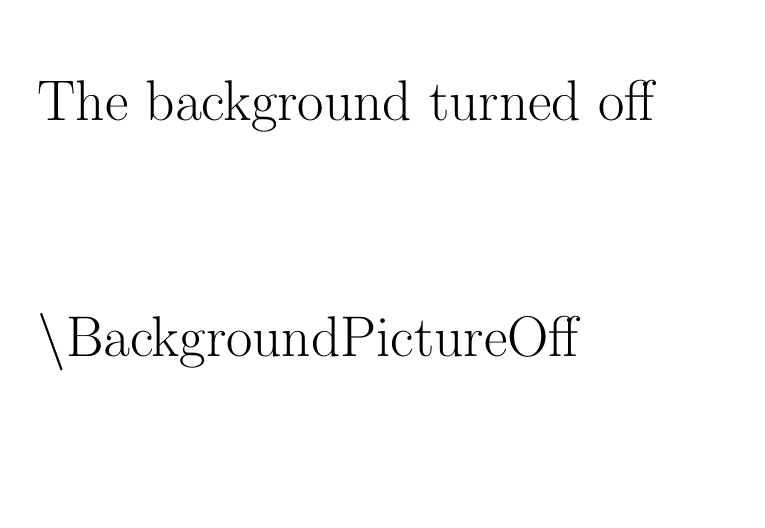
\begin{tikzpicture}
\useasboundingbox (0,0) rectangle (9,6);
\draw[anchor=west] (0,5) node (u) {\fontsize{22}{22}\selectfont The background turned off};
\draw[anchor=west] (0,2) node (u) {\fontsize{22}{22}\selectfont
   $\backslash$BackgroundPictureOff};
\end{tikzpicture}
\end{frame}

\end{document}
